\documentclass[floatsintext, doc]{apa6}
%\bibliography{references}
\usepackage{apacite}
\usepackage{subcaption}
\usepackage{booktabs}
\usepackage{xspace}
\usepackage[utf8]{inputenc}
\usepackage{amsmath}
\usepackage{amssymb}
\usepackage{tikz}
%\usepackage[sc,osf]{mathpazo}
%\linespread{1.12}
\usepackage{booktabs}
\usepackage{centernot}

\usepackage{tikz}
%\usepackage{subfigure}
\usetikzlibrary{bayesnet}

% these packages are needed to insert results 
% obtained from R into the LaTeX document
\usepackage{pgfplotstable}
\usepackage{csvsimple}
\usepackage{siunitx}

% set the name of the folder in which the CSV files with 
% information from R is stored
\newcommand{\datafoldername}{csv_to_tex}


%\makeatletter
%    \let\@internalcite\cite
%    \def\cite{\def\citeauthoryear##1##2{##1, ##2}\@internalcite}
%    \def\shortcite{\def\citeauthoryear##1{##2}\@internalcite}
%    \def\@biblabel#1{\def\citeauthoryear##1##2{##1, ##2}[#1]\hfill}
%\makeatother


% the following code defines the convenience functions
% as described in the main text below

% rlgetvalue returns whatever is the in cell of the CSV file
% be it string or number; it does not format anything
\newcommand{\rlgetvalue}[4]{\csvreader[filter strcmp={\mykey}{#3},
             late after line = {{,}\ }, late after last line = {{}}]
            {\datafoldername/#1}{#2=\mykey,#4=\myvalue}{\myvalue}}

% rlgetvariable is a shortcut for a specific CSV file (myvars.csv) in which
% individual variables that do not belong to a larger chunk can be stored
\newcommand{\rlgetvariable}[1]{\csvreader[]{\datafoldername/myvars.csv}{#1=\myvar}{\myvar}\xspace}

% rlnum format a decimal number
\newcommand{\rlnum}[2]{\num[output-decimal-marker={.},
                             exponent-product = \cdot,
                             round-mode=places,
                             round-precision=#2,
                             group-digits=false]{#1}}

\newcommand{\rlnumsci}[2]{\num[output-decimal-marker={.},
                          scientific-notation = true,
                             exponent-product = \cdot,
                             round-mode=places,
                             round-precision=#2,
                             group-digits=false]{#1}}

\newcommand{\rlgetnum}[5]{\csvreader[filter strcmp={\mykey}{#3},
             late after line = {{,}\ }, late after last line = {{}}]
            {\datafoldername/#1}{#2=\mykey,#4=\myvalue}{\rlnum{\myvalue}{#5}}}

\newcommand{\rlgetnumsci}[5]{\csvreader[filter strcmp={\mykey}{#3},
             late after line = {{,}\ }, late after last line = {{}}]
            {\datafoldername/#1}{#2=\mykey,#4=\myvalue}{\rlnumsci{\myvalue}{#5}}}



\makeatletter
\patchcmd{\epigraph}{\@epitext{#1}}{\itshape\@epitext{#1}}{}{}
\makeatother \def\signed
#1{{\leavevmode\unskip\nobreak\hfil\penalty50\hskip2em
\hbox{}\nobreak\hfil#1% \parfillskip=0pt \finalhyphendemerits=0
\endgraf}} \newsavebox\mybox 

\newenvironment{aquote}[1]
{\savebox\mybox{#1}\begin{quote}} {\signed{\usebox\mybox}\end{quote}}

%\newcommand{\HRule}{\rule{\linewidth}{0.2mm}}



\title{Probabilistic Pragmatics in Syllogistic Reasoning}
\shorttitle{Pragmatics in Syllogistic Reasoning}

\author{Michael Henry Tessler\textsuperscript{1}\textsuperscript{,2}, Joshua B. Tenenbaum\textsuperscript{1}~\& Noah D. Goodman\textsuperscript{2}}
\date{}
  
\affiliation{
\vspace{0.5cm}
\textsuperscript{1} Department of Brain and Cognitive Sciences, Massachusetts Institute of Technology \\
\textsuperscript{2} Department of Psychology, Stanford University
}
%\authorsnames[{1,2},1,2]{Michael Henry Tessler, Joshua B. Tenenbaum, Noah D. Goodman}
%\authorsaffiliations{{Department of Brain and Cognitive Sciences, MIT}, {Department of Psychology, Stanford University}}

\date{}

\usepackage{xcolor}
\usepackage{bbm}

\newcommand{\denote}[1]{\mbox{ $[\![ #1 ]\!]$}}
\newcommand*\diff{\mathop{}\!\mathrm{d}}
\definecolor{Red}{RGB}{255,0,0}
\definecolor{Green}{RGB}{10,200,100}
\definecolor{Blue}{RGB}{10,100,200}

\newcommand{\mht}[1]{{\textcolor{Blue}{[mht: #1]}}}
\newcommand{\ndg}[1]{{\textcolor{Green}{[ndg: #1]}}}
\newcommand{\red}[1]{{\textcolor{Red}{#1}}}

\authornote{Corresponding author: Michael Henry Tessler,  Department of Brain and Cognitive Sciences, Building 46, Room 3027,	Massachusetts Institute of Technology, 77 Massachusetts Avenue, Cambridge, MA 02139-4307, USA; tessler@mit.edu}

\abstract{
Syllogistic reasoning lies at the intriguing intersection of natural and formal reasoning, of language and logic. 
Syllogisms comprise a formal system of reasoning yet make use of natural language quantifiers (e.g., \emph{all}, \emph{some}), and invite natural language conclusions. 
The conclusions people tend to draw from syllogisms deviate substantially from a purely logical perspective. 
Is natural language to blame?
%How can we make sense of the interplay between logic and language? 
\mht{from old abstract:: 
We develop a computational-level theory that considers reasoning over concrete situations, constructed probabilistically by sampling. The base model can be enriched to consider the pragmatics of natural language arguments. The model predictions are compared with behavioral data from a recent meta-analysis. The flexibility of the model is then explored in a data set of syllogisms using the generalized quantifiers most and few. We conclude by relating our model to two extant theories of syllogistic reasoning – Mental Models and Probability Heuristics.}}


\begin{document}
\maketitle


\begin{aquote}{\textbf{Walter J. Ong}, \emph{Orality and Literacy} (1982)}The syllogism is like a text: fixed, boxed-off, isolated... The riddle [by contrast] belongs in the oral world. To solve a riddle, canniness is needed: one draws on knowledge, often deeply subconscious, beyond the words themselves in the riddle. \end{aquote}

%\HRule

\section{Introduction}

In a famous scientific expedition of the 1930s, Russian psychologist Alexander Luria set off into the remote areas of Uzbekistan and Kyrgyzstan in the former Soviet Union to understand the mind of the illiterate peoples of Russia. Among his experiments, Luria would give his participants verbal reasoning problems such as the following:

\begin{quote}
In the Far North, where there is snow, all bears are white. \\
Novaya Zembla is in the Far North and there is always snow there. \\
What color are the bears?
\end{quote}

The kind of response Luria received to such a question depended in part on the literacy of his participant. 
A person who knew how to read and write would respond: ``To go by your words, they should all be white.''
An illiterate person, on the other hand, would say: ``I don't know. I've seen a black bear. I've never seen any others. Each locality has its own animals'' \cite{luria1976cognitive}. 
%Reasoning by appealing to experience or common knowledge, 
Obviously, this is not the answer that Luria had in mind, but what would lead a person to respond in the way that this person did?

%Similar flavors of responses -- appealing to experience or background knowledge -- were found in classic anthropological studies with the Kpelle of Liberia \cite{cole1971cultural, scribner1975recall}.
% A study of American graduate students of the 1960s also uncovered erroneous judgments, and through an analysis of the written protocols of the participants, it was suggested that ``where error occurs, it need not involve faulty reasoning but may be a function of the individual's understanding of the task or materials presented to him'' \cite{henle1962relation}. 

The problem Luria gave his participants resembles a syllogism: a two-sentence argument used to relate two properties (or terms: A, C) via a middle term (B). 
The relations used in classical Aristotelean syllogisms are quantifiers: \emph{all}, \emph{some}, \emph{some .... are not}, and \emph{none}. \footnote{In Luria's syllogism, only one of the premise relations uses a quantifier, so it is not technically an Aristotelean syllogism.} 
An example Aristotelean syllogism reads:

\begin{quote}
All artists are bakers. \\
Some bakers are chemists. \\
\_\_ \\
Some artists are chemists.
\end{quote}

The logical space defined by classical syllogisms is comprised of all combinations of quantifiers and term orders for the premises (e.g., \textsc{quantifier} \textsc{A} -- \textsc{B} vs. \textsc{quantifier} \textsc{B} -- \textsc{A}).
In total, each of the two premises can be appear with one of the four quantifiers and two term orders yielding:  $4$ quantifiers  $\times 2$ term orderings $\times 2$ premises = 64 syllogisms.
Of the 64 unique syllogistic premises, only 27 yield a logically valid conclusion: a conclusion that is true in every situation in which the premises are true.

It is not only the illiterate Soviet peasants of Kyrgyzstan who struggle with reasoning logically with syllogisms.
A recent meta-analysis of syllogistic reasoning tasks performed on American and Italian participants estimated the accuracy of producing a valid conclusion to a logically valid syllogism to range widely (from 90\% to 1\% accuracy) depending on the syllogism \cite{Khemlani2012}.
Logically invalid syllogisms also pose a challenge: the logical response is to conclude that \emph{nothing follows} from the premises (or, report \emph{no valid conclusion}), yet participants readily endorse substantive conclusions for logically invalid syllogisms. 
For example, the syllogism above is not logically valid.  (Consider that it could be only the non-artist bakers that are chemists. In that case, the premises would be true and the conclusion false.)
The conclusion above seems reasonable, however, and roughly 70\% of participants will assert that the \emph{Some As are Cs} conclusion follows from the premises  \cite{Khemlani2012}.
Something beyond logical validity is guiding participants' reasoning behavior. 

% Luria was not the first to study how people reason with syllogisms, and he certainly was not the last. 
% Psychologists have been trying to understand human reasoning with syllogisms for over one hundred years (the earliest experimental study is credited to \citeNP{Storring1908}). 


%In fact, within the confines of the classical syllogism, there is no conclusion about the relation between A \& C that is true in every situation in which the premises are true. 

%Fit into a formal syllogistic form, this argument would read:
%
%Imagine that your friend tells you: ``Everyone in my office has the flu and, you know, some people with this flu are out for weeks.''
%You might respond: ``I hope your officemates are not out for weeks and I hope you don’t get sick either.''
%The form of this exchange resembles a syllogism: 
%
%\begin{enumerate}
%\item \emph{All} officemates are out with the flu (All As are Bs)
%\item \emph{Some} people out with the flu are out for weeks (Some Bs are Cs) 
%\item Therefore, \emph{some} officemates are out for weeks (Some As are Cs)
%\end{enumerate}
%


%people do not seem to find drawing deductively valid conclusions particularly straightforward.

%Faced with such an argument, however, people are perfectly comfortable drawing some conclusion. 
%A meta-analysis of syllogistic reasoning showed that over the population, the proper production of no valid conclusion responses for invalid arguments ranged from 76\% to 12\%. 

% \mht{this is kind of weak, superficial...}
Many theories assume deductive reasoning is the ideal framework by which to evaluate human reasoning  and try to explain reasoning errors as a matter of noise during cognition. 
Errors, then, may arise from improper use of deductive rules \cite{rips1994, geurts2003reasoning} or biased construction of logical models \cite{JL1984, Newstead1992}. 
Probability theory provides an alternative idealized framework by which to evaluate human reasoning, and many other kinds of reasoning are well-explained as probabilistic inference under uncertainty \cite{tenenbaum2006theory}. 

The idealized logical and/or probabilistic framework in which thinking and reasoning unfolds is just part of process of syllogistic reasoning. 
Syllogisms comprise a formal logical system, but they are expressed using the tools of natural language (e.g., they involve natural language quantifiers).
The process of human syllogistic reasoning, thus, involves interpreting and producing natural language sentences; understanding such a task requires a careful examination of the principles of natural language -- semantics and pragmatics -- that may be at play.
Natural language semantics plays a role in many such theories of reasoning \cite{JL1978, Khemlani2012, geurts2003reasoning}, though how pragmatics impacts syllogistic reasoning either remains unclear \cite{Roberts2001} or is posited in an ad-hoc manner \cite{Chater1999}. 


%Errors may occur with respect to any idealized theory but they need not be explained as faulty reasoning that framework.
%Rather, the participant's understanding of the task  -- of what is being asked of them -- may instead be cause of supposed errors \cite{henle1962relation}. 

In this paper, we explore the idea that syllogistic reasoning is part logical reasoning and part riddle solving (as suggested by the Ong, 1982 quotation above).
Concretely, we view syllogistic reasoning as involving two language understanding tasks \cite<cf.>{geurts2003reasoning}: interpreting the premises of the syllogism and producing a conclusion.
Each of these component tasks could involve pragmatic reasoning beyond the words of the syllogism \cite{Grice1975, Clark1996, Levinson2000}. 
We formalize this reasoning in a probabilistic model of pragmatic reasoning in the Rational Speech Act framework \cite{Frank2012a, goodman2016pragmatic}.
We show that interpreting the premises of a syllogism offers multiple, distinct varieties of pragmatic reasoning.
In particular, the structure of the syllogism could induce a kind of pragmatic reasoning that is distinct from standard, scalar-implicature type reasoning (as explored in \citeNP{Roberts2001}), reasoning that is more akin to riddle solving. 
We formalize this notion as a Question Under Discussion \cite{Roberts2004QUD}, in which a listener reasons about the conclusion a speaker intended the listener (or, reasoner) to draw from the syllogism. 
%This reasoning is more akin to riddle solving: Reasoning about what conclusion a speaker intended the listener (or, reasoner) to draw from the syllogism. 
We formalize this hypothesis and alternative hypotheses in models that we test against a recently collected data set of human reasoning with syllogisms. 


%``where error occurs, it need not involve faulty reasoning bu
%of human syllogistic reasoning

% provides a natural description of a world in which you don’t know exactly how many people are in your office are going to get the flu.

% A separate dimension of theories of human reasoning concerns the extent to which principles of natural language — semantics and pragmatics — are necessary for understanding reasoning tasks. 



% the idea that pragmatic reasoning operating on top of probabilistically constructed models of situations can provide insight into how people reason with syllogisms.
%We develop a set of models that vary in how they interpret the premises of the syllogism and decide upon a conclusion that follows.
%In particular, we explore 
%reasons about multiple quantifier sentences to produce a distribution over conclusions that follow from those sentences. 
%\mht{deprecated:: We present three sets of results, highlighting the influence of different components of the model on human reasoning: (1) the influence of prior beliefs; (2) flexibility in natural language semantics, incorporating generalized quantifiers (e.g., “most” and “few”); and (3) pragmatic rea- soning. Previous approaches to the pragmatics of syllogistic reasoning have reduced the interpretations of syllogistic arguments to the interpretations of the individual premises or quantifiers used in those premises \cite{Roberts2001}. For example, premises involving the quantifier “some” may be interpreted as implying some but not all. But that sort of reasoning will not produce the conclusion in the syllogism above. Instead, what is needed is a richer scope of pragmatic reasoning: Reasoning about why about the speaker constructed the argument as a whole. We formalize this notion as a Question Under Discussion (C. Roberts, 2004) in which a listener reasons about the most likely conclusion (i.e., A–C relation) given the premises heard. We find that this formulation of pragmatic reasoning is able to break critical symmetries that would result from logical reasoning (Figure 1). An early version of this model was presented by Tessler and Goodman (2014).}


%Cognitive theories of human reasoning turn along the critical dimension of whether the core ideal of reasoning is deductive validity or probabilistic support. 
%
%
%This cartoon illustrates a critical dimension along which cognitive theories of reason- ing differ: whether the core and ideal of reasoning is deduc- tive validity or probabilistic support. 
%
%
%An important extension to baseline CPT frameworks concerns incorporating pragmatics and language-like properties (such as compositionality) and representations in probabilistic inference. The probabilistic programming language (PPL) / probabilistic language of thought (PLoT) can more naturally apply to richer forms of reasoning, including everyday reasoning under uncertainty (e.g., Goodman et al., 2015). Furthermore, enriching these models with an understanding of natural language pragmatics can explain apparent fallacies in classical reasoning tasks (e.g., Tessler \& Goodman, 2014). Assuming a communicative context to a task involving language allows a reasoner in a PPL/PLoT model to incorporate the goals of a speaker (e.g., assuming the speaker intends to be informative), so providing a rational perspective on reasoning fallacies. We will also consider the way resource limitations guide practical models in PPL.
%
%
%
%
%By formalizing syllogistic reasoning as a probabilistic pragmatics problem, there is a natural way to account for influence of background knowledge in the form of the prior distribution on possible situations. We construct domains where we expect correlations between properties (e.g., knives – being sharp – cut well) and investigate syllogistic reasoning over these content domains. By measuring the prior probability of the eight possible combinations of binary features, we are able to generate predictions for syllogistic reasoning problems that are influenced by this kind of prior knowledge. Such influence of background knowledge on reasoning, known as belief bias in the syllogistic reasoning domain, has been of interest to psychologists for quite some time (e.g., Evans, Handley, \& Pollard, 1983; Dube, Rotello, \& Heit, 2010). We formalize this “bias” as rational belief updating given prior knowledge and find that the pragmatics model is too influenced by these kind of prior beliefs (Figure 2).


\section{Computational Model}

%\section{Bayesian argument strength in syllogistic reasoning}

Syllogistic reasoning involves two language understanding tasks: interpreting the premises of the syllogism and producing a conclusion.
Each of these components could involve some kind of pragmatic reasoning.
Our model uses recursive Bayesian reasoning that grounds out in a literal listener model who updates their beliefs about the state of the world given the literal (logical) meaning of the utterances. 
We walk through our ontology of the state space and the literal meanings before describing the different models of premise interpretation and conclusion production. 


\subsection{Ontology and semantics}

The model is based on an ontology of situations represented by Venn diagrams corresponding to all possible logical relations between the sets of three properties: A, B, C. 

\begin{figure}[h]
\centering
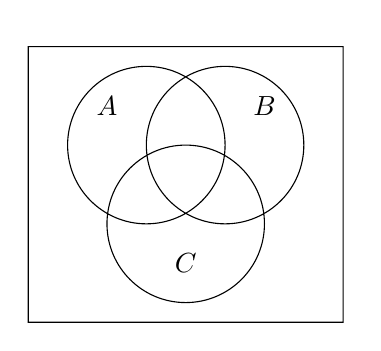
\begin{tikzpicture}[fill=gray]
% left hand
%\scope
%\clip (-2,-2) rectangle (2,2)
%      (1,0) circle (1);
%\fill (0,0) circle (1);
%\endscope
% right hand
%\scope
%\clip (-2,-2) rectangle (2,2)
%      (0,0) circle (1);
%\fill (1,0) circle (1);
%\endscope
% outline
\draw (0,0) circle (1) (-0.5,0.25)  node [text=black,above] {$A$}
      (1,0) circle (1) (1.5, 0.25)  node [text=black,above] {$B$}
      (0.5,-1) circle (1) (0.5,-1.25)  node [text=black,below] {$C$}
      (-1.5,-2.25) rectangle (2.5,1.25) node [text=black,above] {};
\end{tikzpicture}
\label{fig:venn}
\caption{A state is represented by Boolean values over the regions of a Venn diagram, corresponding to the presence or absence of unique object types.}
\end{figure}

Each Venn diagram contains eight regions $i \in R$, corresponding to the presence or absence of each of the three properties: $\{\{A,B,C\},$ $\{A,B,\neg C\},$ $\{A,\neg B,C\},$ $\{\neg A, B, C\},$ $\{A, \neg B, \neg C\},...\}$. (For simplicity, when possible, we will refer to regions by the properties that are present, omitting the absent properties; for example, $\{A, B, \neg C\}$ will be referred to as $AB$.)
These regions can be thought of as unique object types (e.g., an object defined by having properties $A$ and $B$ but not $C$.\footnote{This diagram representation is analogous to a mental model in the style of \citeA{johnson1983mental} composed of object tokens (e.g., some objects which have properties $A$ or $B$, etc.) but where only unique object tokens are represented (e.g., there cannot be two objects which have the same set of properties).}
The empty region (or, the object type which has neither of the three properties: $\{\neg A, \neg B, \neg C\}$) does not impact the truth conditions of the quantifier sentences used in syllogisms, and hence, we omit this region and model only seven regions.
Then, a situation (Venn diagram) $s \in S$ is composed of the set of object types (regions) that are present (e.g., $\{AB, BC, A\}$ is one possible state).
The set of unique states has size $2^7 = 128$.
%, though we exclude the state where all eight regions are empty (i.e., the state where there are no As, Bs, and Cs, but also no things that are not As, Bs, or Cs).

Our model probabilistically generates states $s \in S$ by sampling a Bernoulli random variable for each of the $i \in R$ regions. 

$$P(s) = \prod_{i \in R} P(A_{i}, B_{i}, C_{i}) $$%= (P(a) \cdot P(b) \cdot P(c)) ^n$$

%\subsection{Semantics}
The classical syllogisms are comprised by two premise arguments where each premise relates two properties via a quantifier. 
The quantifiers in classical syllogism are \emph{all}, \emph{some}, \emph{none}, and \emph{not all}.\footnote{
These quantifiers are typically presented in sentences such that \emph{none} is rendered as \emph{no} (e.g., No As are Bs) and \emph{not all} is rendered as \emph{some \_\_ are not} (e.g., Some As are not Bs).
}
We use the classic logical semantics of these quantifiers described in Table \ref{tab:sem}.
\mht{CHECK THIS:
We assume the statements involving \emph{all} and \emph{none} describe situations in which there exist objects that have the property, sometimes referred to as the ``existential presupposition'' (e.g., \emph{All A are B} is false if there are no As). 
}
%: \emph{All As are Bs} entails that $\nexists (A \& \neg B)$;  \emph{Some As are Bs} entails that $\exists (A \& B)$; \emph{Some As are not Bs} entails that $\exists (A \& \neg B)$; \emph{No As are Bs} entails that $\nexists (A \& B)$.


% Please add the following required packages to your document preamble:
%\begin{table}[]
%\centering
%\begin{tabular}{@{}lll@{}}
%\toprule
%Example syllogistic sentence & Consistent State & Inconsistent state \\ \midrule
%All As are Bs                & \{AB, ABC\}      & \{A, ABC\}         \\
%Some As are Bs               & \{A, AB\}        & \{A, AC\}          \\
%Some As are not Bs           & \{A, AB\}        & \{AB, ABC\}        \\
%No As are Bs                 & \{A, AC\}        & \{A, AB\}          \\ \bottomrule
%\end{tabular}
%\caption{cap}
%\end{table}


% Please add the following required packages to your document preamble:
% \usepackage{booktabs}
\begin{table}[]
\begin{tabular}{@{}llll@{}}
\toprule
Example syllogistic sentence & Literal Meaning                                                                       & Consistent State & Inconsistent state \\ \midrule
All As are Bs                                      & $\forall i \in R: A(i) \implies B(i) $ & \{AB, ABC\}                           & \{A, ABC\}                              \\
Some As are Bs                                     & $\exists i \in R: A(i) \implies B(i) $ & \{A, AB\}                             & \{A, AC\}                               \\
Some As are not Bs                                 & $\exists i \in R: A(i)  \centernot \implies B(i) $ & \{A, AB\}                             & \{AB, ABC\}                             \\
No As are Bs                                       & $\forall i \in R: A(i) \centernot \implies B(i) $  & \{A, AC\}                             & \{A, AB\} \\ \bottomrule
\end{tabular}
\caption{Literal meanings of example syllogistic sentences with examples of states that are consistent with the literal meanings and inconsistent with the literal meanings.}
\label{tab:sem}
\end{table}

\subsection{Interpreting the premises}

Given a representation and assignment of prior probabilities to different states (Venn diagrams), we now introduce probabilistic listener models that update their beliefs about the states given the premises of the syllogism. 
This interpretation process can occur at the level of a literal listener (who updates beliefs based on the truth-conditional meaning of the premises) or a pragmatic listener who interprets the premises by reasoning about why a speaker chose to produce the premises that she did. 

\subsubsection{Literal interpretation of premises}

All our recursive reasoning modeling components ground out in a model of literal interpretation.
This model component is a Bayesian literal listener $L_0$ which updates its prior beliefs about the state via the literal, truth conditional meaning of the utterance (shown in Table \ref{tab:sem}):

\begin{equation}
L_0(s \mid u ) \propto P(s)\cdot \mathcal{L}(u, s) 
\label{eq:L0}
\end{equation}
\noindent where $\mathcal{L}(u, s)$ is the lexicon that encodes the literal meanings of the quantified utterances used in syllogisms. 
These meanings can resolve to deterministic outcomes (e.g., $\mathcal{L}(u, s) = 1$ if the utterance $u$ is true of $s$, and 0 otherwise). 
In practice, however, we assume a small amount of noise $\phi$ in the semantics such that $\mathcal{L}(u, s) = 1$ with probability proportional to $1-\phi$ and if the utterance $u$ is true of $s$.
In other words, we assume a continuously valued semantics such that $\mathcal{L}(u, s) \in [0, 1] \subset \mathbb{R}$ as introduced by \citeA{degen2020redundancy}.

The model of literal interpretation can be used to update the prior distribution on states (Venn diagrams) into a posterior distribution given the meaning of the premises of the syllogism. 
For the interpretation of a syllogism, $u$ is composed of two utterances (the two syllogistic sentences): $u_1$ and $u_2$. 
Belief updating proceeds by assuming both utterances are true: 
\begin{equation}
L_0(s \mid u_1,  u_2) \propto P(s)\cdot \mathcal{L}(u_1, s) \cdot \mathcal{L}(u_2, s) 
\label{eq:L0premises}
\end{equation}

Equation \ref{eq:L0premises} defines a probability distribution over states (Venn diagrams) given the premises of the syllogism. 
Logically valid syllogisms given rise to a distribution over states where a quantifier relationship between the conclusion terms of the syllogism are true in all possible states given the premises. 
For example, in the logically valid syllogism  \emph{All As are Bs}, \emph{All Bs are Cs} (the ``Barbara'' syllogism), the relationship \emph{All As are Cs} is true in every possible state in which the premises are true; in particular, the region \emph{ABC} (an object which has all three properties) is true in every possible state (Figure \ref{fig:AAvenns}).
On the other hand, the premises of logically invalid syllogisms tend to give rise to many possible states in which no particular syllogistic conclusion is true in every state; some conclusions are true in more states, however, than other conclusions.
For example, in the logically invalid \emph{No As are Bs}, \emph{Some Bs are Cs}, the conclusion \emph{All As are Cs} is logically possible though is true in fewer states than \emph{No As are Cs} (Figure \ref{fig:EIvenns}).


\begin{figure}[t]
\centering
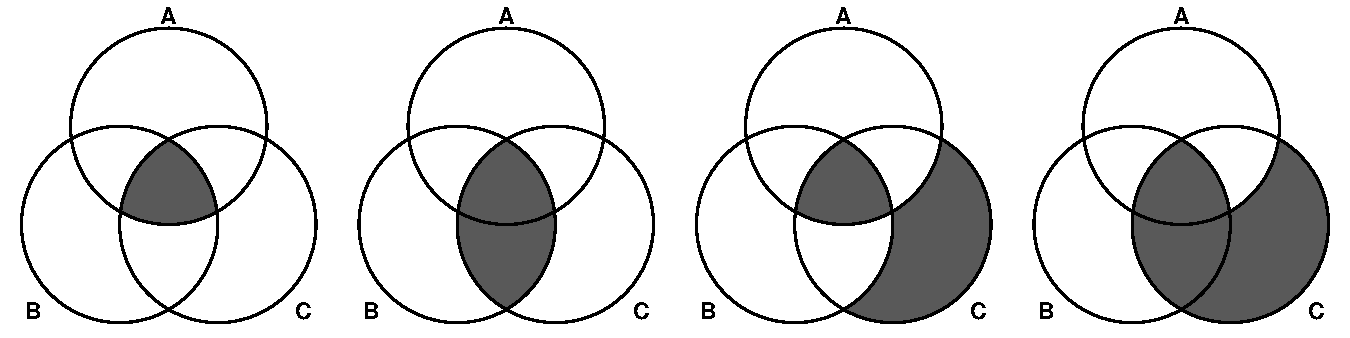
\includegraphics[width = \textwidth]{figs/diagrams_allAB_allBC.pdf}
\caption{Set of Venn diagrams (states) literally compatible with the premises of the logically valid syllogism: \emph{All As are Bs}, \emph{All Bs are Cs}. The conclusion relation \emph{All As are Cs} is true in every compatible state.}
\label{fig:AAvenns}
\end{figure}



\begin{figure}[b!]
\centering
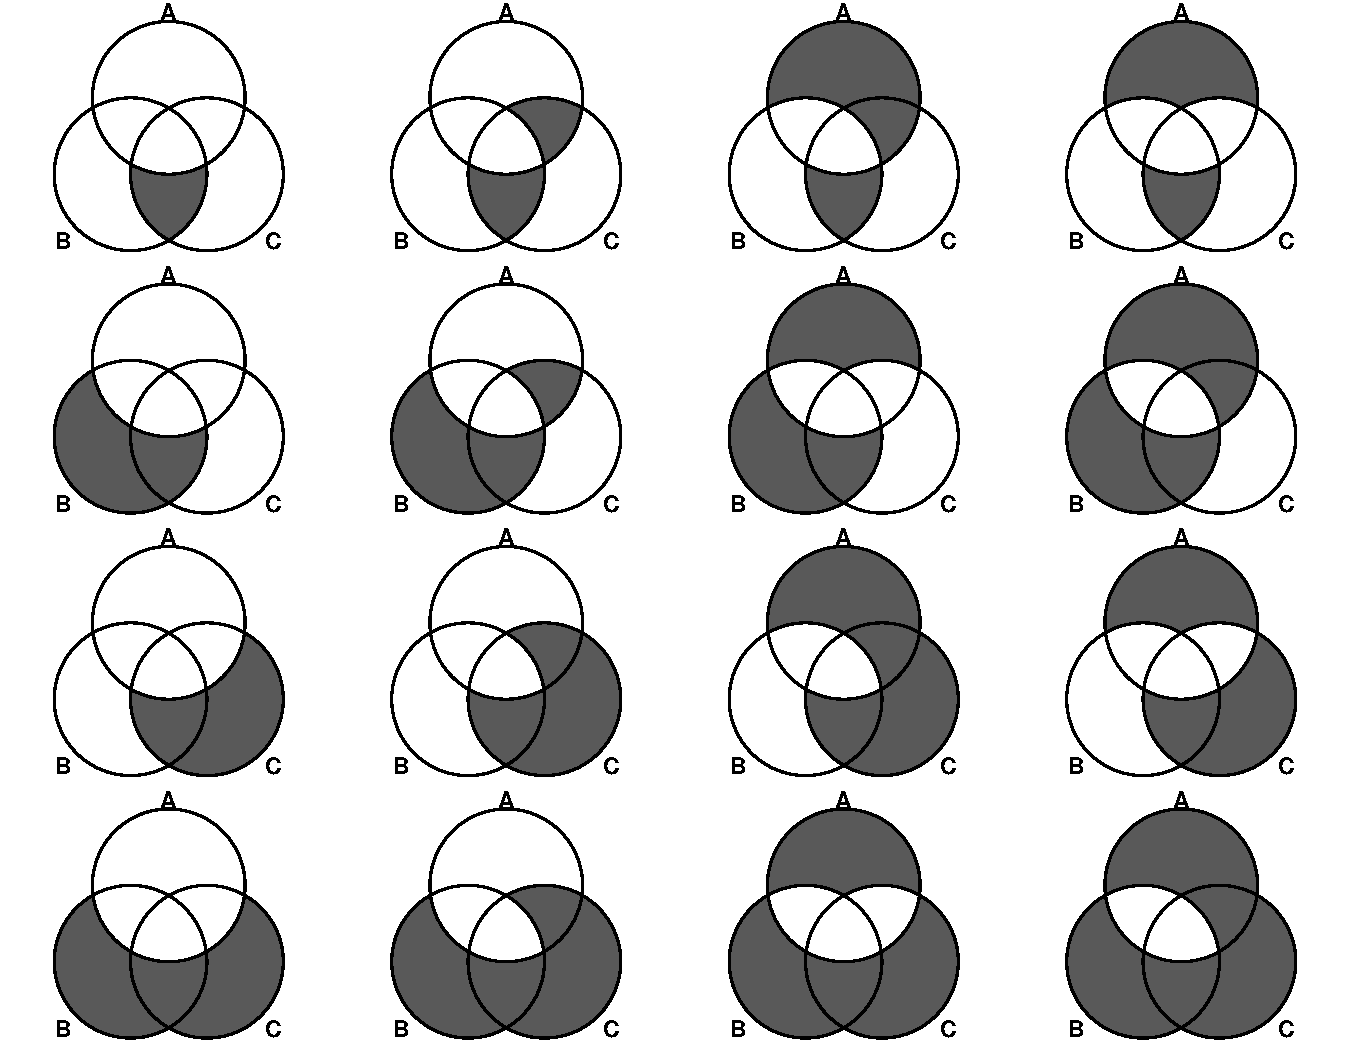
\includegraphics[width = \textwidth]{figs/diagrams_noneAB_someBC.pdf}
\caption{Set of Venn diagrams (states) literally compatible with the premises of the logically invalid syllogism: \emph{No As are Bs}, \emph{Some Bs are Cs}. No syllogistic conclusion is true in every compatible state.}
\label{fig:EIvenns}
\end{figure}


\subsubsection{Pragmatic interpretation of premises}

Understanding language often involves reasoning not only about the literal meaning of what was said but about why an interlocutor (the speaker) would bother to say what they said, which can lead to enriched interpretations beyond the literal meanings. 
We can formalize this reasoning through a series of Bayesian models that recursively reason about one another, as developed in the Rational Speech Act (RSA) framework \cite{Frank2012a, goodman2016pragmatic, scontras2018probabilistic}.
Concretely, we describe a pragmatic listener $L_1$ who reasons about a speaker $S_1$ who produces utterances in order to convey information to the literal listener (Equation \ref{eq:L0premises}):

\begin{align}
L_1(s \mid u_1,  u_2)& \propto  P(s)\cdot S_1(u_1, u_2 \mid s)  \label{eq:L1} \\ 
S_1(u_1, u_2 \mid s) &\propto  \exp [ \alpha_1 \cdot \ln L_0(s \mid u_1,  u_2)]  \label{eq:S1}
\end{align}

The definition of the pragmatic listener (Equation \ref{eq:L1}) mirrors that of the literal listener (Equation \ref{eq:L0}) except in that the likelihood is defined as the probability that a speaker $S_1$ would produce utterances (premises) $u_1$ and $u_2$ given a state $s$.
Following standard practice in RSA modeling, the speaker is a soft-max rational agent (with degree of rationality $\alpha_1$) who produces utterances in order to convey information about the state $s$ to the literal listener.
The normalization in Equation \ref{eq:S1} implies a normalization over a set of alternative utterances (i.e., the set of sentences that the speaker could have, but didn't, produce); in order case, the set of alternative utterances amounts to a set of alternative syllogistic premises that a speaker could have produced. 
There are at least three sets of alternative premises that are \emph{a priori} plausible and we test our models on all three: (1) alternative premises that have the same ordering of terms (i.e., syllogisms of the same \emph{figure}), but whose quantified relation between the terms could be different (e.g., if the speaker says \emph{All As are Bs. All Bs are Cs.}, the alternative set is the set of syllogisms of the form \emph{Q As are Bs}. \emph{Q Bs are Cs.} where $Q \in \{all, some, \emph{not all}, none\}$); (2) alternative premises that differ either in the quantified relation between terms or the ordering of the terms, but not both (i.e., utterances with an edit-distance of 1); (3) the maximal set of alternative premises in which the quantifier and the ordering of terms could be different.


%\mht{OPEN QUESTION being explored with modeling... what alternative utterances to use for the speaker:}
%Here we assume that the alternative set is all syllogisms with the same ordering of terms 
\subsection{Producing a conclusion}

The second component of a syllogistic reasoning model is a model of conclusion production. 
That is, given an a set of beliefs about the likely state of affairs (Venn diagrams), what conclusion should be drawn?
We formalize two models of conclusion production.
The first is a literal speaker, who selects conclusions that are likely to be true given the speaker's beliefs about the state. 
The second is a pragmatic speaker, who selects a conclusion that would best align a naive listener's beliefs about the state with the beliefs of the speaker.
Since these models produce a distribution over conclusions, we label these models as reasoner models $R$, so as to not confuse them with the speaker models $S$ that are used as part of the recursion in the pragmatic interpretation of premises.
%The pragmatic production of a conclusion is a model of a speaker who tries to produce the most informative utterance (conclusion) to convey information to a naive listener. 

\subsubsection{Space of conclusions}

The syllogistic reasoning task presents participants with a set of options for the quantifier relationship between the two terms of the syllogisms that are not described explicitly in relation to each other in the premises (i.e., the terms \emph{A} and \emph{C} if the premises are of the form \emph{A -- B}, \emph{B -- C}.). 
Particular tasks differ in the set of options that are given to participants, but the maximal includes the four quantifiers  (\emph{all}, \emph{some}, \emph{not all}, \emph{none}) crossed with the two orderings of the terms of the conclusion (i.e., \emph{A -- C} or \emph{C -- A}).
Thus, there are eight contentful conclusion options. 

A ninth unique option, however, is also available: the option that \emph{nothing follows} (sometimes described \emph{no valid conclusion}). 
The \emph{nothing follows} conclusion is the logically correct answer for the logically invalid syllogisms and is produced to variable extents in both logically valid and invalid syllogisms \cite{Khemlani2012}.
While the semantics of the quantifier conclusions are quite clear, the proper treatment of the \emph{nothing follows} conclusion is not obvious. 
Extant theories treat this option indirectly, either as a byproduct or last resort of a reasoning process, when it is treated at all \cite{ragni2019does, riesterer2020modeling}.
We approach the question of the meaning of \emph{nothing follows} from a language production standpoint, where the statement is tantamount to not saying anything at all. 
Therefore, we model the \emph{nothing follows} statement as one that is true in every possible state of affairs, and hence does not update a listener's beliefs about the state. 
% From a language production perspective, however, the


\subsubsection{Literal production of conclusions}

% In a classical reasoning model, these 
% lexical meanings such that
% Our pragmatics model begins with submodal that performs a literal interpretation of the premises. 
% The model computes a 
Given a belief updating model based on the premises of a syllogism $L$ (either literal $L_0$ or pragmatic $L_1$), we can define a literal production model $R_0$ that uses the listener $L$'s posterior distribution on states to determine what conclusion is likely to be true given the premises. 
This model $R_0$ can be viewed as one that is sampling a state from the listener's posterior distribution on states and randomly choosing among the conclusions that are literally true of that state. 

%The strength of a syllogistic argument (two premises) for a conclusion is a real-valued number between 0 and 1 given by the $P(u_c \mid u_1, u_2)$, where $u_1$ and $u_2$ are the two premises of the syllogism.

\begin{equation}
R_0(u_3 \mid u_1, u_2) \propto \sum_s \mathcal{L}(u_3, s) \cdot L(s \mid u_1, u_2) \label{eq:R0}
\end{equation}

\subsubsection{Informative production of conclusions}

Just as with our submodel of premise interpretation, we can define a reasoner model who selects conclusions in order to convey information to a naive listener (who has heard neither premises nor conclusion). 
Since the reasoner does not know the state (but only has beliefs about the state given the premises of the syllogism), we operationalize the informational utility of a conclusion by how well it would align the listener's beliefs with those of the reasoner. 
Formally, we use the information-theoretic measure of Kullback-Leibler (KL) divergence as the measure of alignment of the naive listener and reasoner's belief distributions. 
Again, this formalization is agnostic as to how we compute the reasoner's state distribution (whether it be via a literal or a pragmatic interpretation of the premises), and so we denote the reasoner's belief distribution over the state as $R$.

\begin{align}
  \label{eq:KL-divergence}
  \text{KL}({R \mid \mid L_0}(u)) = - \sum_{s} R(s) \ \log \frac{R(s)}{{L_{0}}(s \mid u)}
\end{align}

\noindent Then, the reasoner model that selects conclusions an informative manner is given by: 

\begin{equation}
R_1(u_3 \mid u_1,  u_2) \propto  \exp [ \alpha_2 \cdot \text{KL}({R_1(s) \mid \mid L_0}(s \mid u)) ]  \label{eq:R1}
\end{equation}

\noindent where $L_0(s \mid u)$ is the literal listener model defined in Equation \ref{eq:L0}. 
%prior distribution over situations with the literal meanings of the quantified statements: 






%Using KL-divergence, we can then state a more general definition of utterance utilities, to
%replace \eqref{U}:
%\begin{align}
%  \label{eq:Utils-KL-based}
%  U_{S_1}(u; s) = \text{KL}(P_{S_{1}\text{-}Bel} \mid \mid P_{L_{0}\text{-}Bel}(u)) - C(u)
%\end{align}


\section{Modeling the Ragni et al. (2019) data set}

We test our model using a dataset published by \citeA{ragni2019does}. The data set consists of the results of a web experiment in which participants ($n = 139$) provided conclusions to all 64 syllogisms. In the experiment, participants completed all syllogistic reasoning problems after a brief training phase. Participants responded by selecting one of the nine possible responses for the conclusion of the syllogism (4 quantifier choices x 2 term orders + 1 \emph{nothing follows}).
Participants' responses to four example syllogisms are shown in Figure \ref{fig:ragniData}).

%\begin{figure}[th]
%\centering
%\includegraphics[width = \textwidth]{figs/ragni_4sylls.pdf}
%\caption{Human conclusion choices for four syllogistic reasoning problems from the \citeA{ragni2019does} data set.}
%\label{fig:ragniData}
%\end{figure}



\subsection{Bayesian data analysis}

To assess how well our models can accommodate the syllogistic reasoning data from \citeA{ragni2019does}, we embed each model variant within a Bayesian data analysis model to infer the credible values of the latent parameters of the models and generate predictions given those parameters. 

\subsubsection{Parameters and priors}

We parametrize the prior distribution over states (Venn diagrams) $P(x)$ in the reasoner models via independent Bernoulli random variables $\theta_k$ corresponding to the prior probability of each of the seven regions of a Venn diagram; we put uniform priors over the unit interval for these parameters.
We assume a small amount of noise in the literal semantics of the utterances such that with a small probability $\phi$, the literal listener disregards the utterance heard and does not update its beliefs via that utterance; we put a uniform prior over the limited range of (0, 0.1) over this parameter since we assume the noise to be a small quantity. 

We assume two global variables that modulate the pragmatic reasoner's prior preferences for certain conclusions. 
The conclusion prior is parameterized by unnormalized probability weights, where a uniform prior would have a weight of 1 for all conclusions. 
The first parameter is a global preference or dispreference $\beta_0$ for the \emph{nothing follows} conclusion; we put a uniform prior between (0, 2) on this weight. 
The second is a global preference  $\beta_1$ for conclusions whose order of the terms (A--C vs. C--A) matches the order of the terms in the premises; we put a uniform prior between (1, 5) on this weight since we assume it to be preference for producing conclusions that match the order of the terms of the syllogism. 
This first term preferences works by checking whether either A or C appear in the subject position of the premise.
If only one appears in the subject (e.g., the syllogistic frame \emph{A--B/B--C}), then conclusions where that same term appears in the subject (e.g., \emph{A--C}) will have a bias determined by $\beta_1$.
If both or neither appear in the subject (e.g., \emph{A--B/C--B} or \emph{B--A/B--C}), then no preference is given in the conclusion prior, corresponding to an unnormalized probability weight of 1. 

Finally, the Rational Speech Act modeling framework assumes speakers are approximately rational agents who produce utterances as actions whose utility is defined by conveying information to a listener. The degree of rationality of the speaker interpolates between probability matching behavior and utility maximizing behavior. 
In our model, we have two speaker components: one involved in the pragmatic interpretation of the premises and one involved in the pragmatic production of conclusions; each of these carries with a speaker optimality parameter $\alpha$. 
For these parameters, we assume uniform priors over the range of (0, 20), consistent with the prior literature on RSA models. 


\begin{figure}[ht!]
\begin{center}
\begin{tabular}{cc}
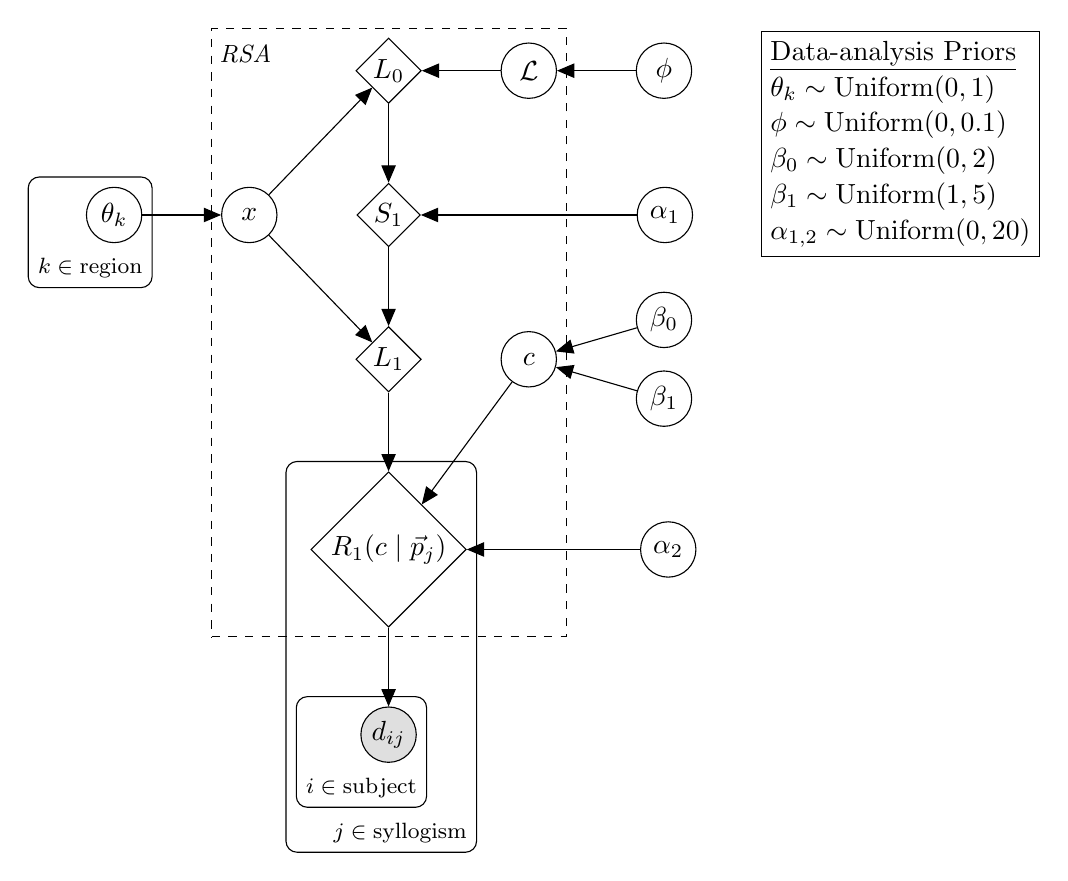
\begin{tikzpicture}
%% RSA nodes and data
\node[obs](data){$d_{ij}$};

\node[det, above=of data](R1){$R_{1}(c \mid \vec{p}_j)$};
\node[det, above=of R1](L1){$L_{1}$};
\node[det, above=of L1](S1){$S_{1}$};
\node[det, above=of S1](L0){$L_{0}$};

\node[latent, left=of S1](x){$x$};
\node[latent, left=of x](theta){$\theta_k$};

\node[latent, right=of L0](lex){$\mathcal{L}$};
\node[latent, right=of lex](phi){$\phi$};

\node[latent, right=of S1, xshift=1.74cm](alpha1){$\alpha_1$};

\node[latent, right=of L1](c){$c$};
\node[latent, right=of c, yshift = 0.5cm](b0){$\beta_0$};
\node[latent, right=of c, yshift = -0.5cm](b1){$\beta_1$};

\node[latent, right=of R1, xshift=1.2cm](alpha2){$\alpha_2$};

\gate {RSAgate} {(R1)(L1)(S1)(L0)(lex)(x)(c)} {} ; %

\plate{plate_region}{(theta)}{$k \in \text{region}$};
\plate{plate_data}{(data)}{$i \in \text{subject}$};

\plate{plate_syllogism}{
 (R1)(data)(plate_data)
}{$j \in \text{syllogism}$}


\edge{R1}{data};
\edge{L1}{R1};
\edge{S1}{L1};
\edge{L0}{S1};

\edge{theta}{x};

\edge{x}{L0};
\edge{x}{L1};

\edge{lex}{L0};
\edge{phi}{lex};

\edge{alpha1}{S1};

\edge{c}{R1};
\edge{b0}{c};
\edge{b1}{c};

\edge{alpha2}{R1};

\node[text width=1cm] at (-1.65,8.65) {\emph{\small{RSA}}};

\node[draw, align=left, execute at begin node=\setlength{\baselineskip}{3ex}] at (6.5, 7.5) { 
\text{\underline{Data-analysis Priors} } \\ 
$ \theta_k  \sim \text{Uniform}(0, 1)$ \\
$ \phi  \sim \text{Uniform}(0, 0.1)$ \\
$ \beta_0  \sim \text{Uniform}(0, 2)$ \\
$ \beta_1  \sim \text{Uniform}(1, 5)$ \\
$ \alpha_{1, 2}  \sim \text{Uniform}(0, 20)$ 
};

%$\beta^\rho_0 ,\beta^\rho_1 \sim \text{Uniform}(-2,2)$ \\
% $\rho_i = \text{logistic}(\beta^\rho_0  + i \cdot \beta^\alpha_1)$ \\
% $d^{CG}_{i} \sim \text{Bernoulli}(\rho_i)$ \\
% \\
%$\beta^\alpha_0 \sim \text{Uniform}(-3,3); \beta^\alpha_1 \sim \text{Uniform}(-0,4)$ \\
% $\alpha_i = \beta^\alpha_0  + i \cdot \beta^\alpha_1$ \\
% \\
% $\mu^\theta_0 \sim \text{Uniform}(-3,3); \mu^\theta_1 \sim \text{Uniform}(0,2)$ \\
% $\sigma^\theta_0 \sim \text{Uniform}(0,2); \sigma^\theta_1 \sim \text{Uniform}(0,1)$ \\
% $\beta^\theta_0 \sim \text{Gaussian}(\mu^\theta_0, \mu^\sigma_0); \beta^\theta_1 \sim \text{Gaussian}(\mu^\theta_1, \mu^\sigma_1)$  \\
% $\theta_{ij} = \text{logistic}(\beta^\theta_{0,j}  + i \cdot \beta^\theta_{1,j})$ \\
% $d^{ME}_{ij} \sim L'_{ij},  d^{CM}_{ij} \sim L_{ijk}$
%};
%
%\node[draw, align=left, execute at begin node=\setlength{\baselineskip}{3ex}] at (8,0) {Integration model\\ $P_{L_{1}}(r \mid u; \{\rho_i, \alpha_i\, \theta_{ij}\})\propto P_{S}(u \mid r; \{\alpha_i, \theta_{ij}\}) \cdot P(r \mid \rho_i) $\\ 
%$P_{S}(u \mid r; \{\alpha_i\, \theta_{ij}\})\propto P(r \mid u; \{\theta_{ij}\}) ^{\alpha_i} $\\
%$P(r \mid u; \{\theta_{ij}\}) \propto \mathcal{L}(u, r \mid \theta_{ij})$
%};


\end{tikzpicture}

    \end{tabular}
  \end{center}
  \caption{\small Bayesian data analysis model. The conclusion choices for each $i$ participant on each $j$ syllogism $d_{ij}$ are generated via the pragmatic reasoner model $R_1$, which defines a conditional distribution on conclusions $c$ given premises $\vec{p}_j$. The reasoner model $R_1$ is a Rational Speech-Act (RSA) model that interprets premises according to a pragmatic listener model $L_1$, who reasons about a speaker $S_0$ who reasons about a literal listener $L_0$ which updates its beliefs according to the literal meaning $\mathcal{L}$ of the sentences it hears. Literal meanings are the standard, truth-functional meanings of the quantifiers (Table 1\label{tab:sem}) with a small amount of noise $\phi$. The prior distribution over states $P(x)$ is parameterized by independent Bernoulli weights $\theta_k$ for each of the 7 $k$ regions of a Venn diagram. The reasoner $R_1$'s prior distribution over conclusions includes a preference $\beta_1$ for term-orderings (A--C vs. C--A) that match the ordering of the terms in the premises; in addition, the prior includes a separate baseline weight for the \emph{nothing follows} conclusion $\beta_0$. Finally, the speaker components of the model---both the speaker $S_1$ which plays a role in the pragmatic interpretation of the premises and the reasoner $R_1$ that selects conclusions in a pragmatic fashion---have independent soft-max parameters $\alpha$.}
  \label{fig:bayesnet}
\end{figure}

\subsubsection{Implementation and inference}

We implemented the cognitive models and the Bayesian data analytic models in the probabilistic programming language WebPPL \cite{dippl}. 
To learn about the credible values of the parameters, we ran 3 MCMC chains each for 15,000 iterations discarding the first 5,000 iterations for burn-in. 
We assessed convergence through visual comparison of the posterior distributions to ensure that the inferences that resulted from looking at different chains were not appreciably different.

\subsubsection{Results}

\paragraph{Posterior predictive checks}

\paragraph{Posterior on parameters}

\paragraph{Model comparison}




\section{Experiments}

\section{Discussion}

\citeA{Roberts2001} explore the predictions of logic-based accounts in which the quantifiers \emph{some} and \emph{some are not} are interpreted in a Gricean fashion (e.g., \emph{some} pragmatically entail $\neg \forall$) and found that this alone is not sufficient to explain human reasoning with syllogisms. 
Our approach differs from their in a number of important respects.
Foremost, in our model, scalar implicature as an all-or-nothing phenomenon; instead, implicatures emerge probabilistically via Bayesian social reasoning, wherein a listener reasons about what else an approximately rational speaker could have said. 
This probabilistic treatment of pragmatic reasoning has two effects: (i) \emph{some} does not necessarily imply $\neg \forall$ and (ii) the interpretations of \emph{some A are B} and \emph{some A are not B} are not equivalent (contra the treatment in \citeNP{Roberts2001}).
Second, we introduce the idea that the syllogistic reasoning task presents a particular Question Under Discussion (QUD) which can alter the pragmatic enrichments that alter the literal meaning of the premises in a syllogism; in particular, the syllogism introduces the \textsc{AC} QUD (``what is the relation between A and C?'' ), which invites the listener to weight the evidence for a particular conclusion from the current syllogism in the space of possible syllogisms. 
Finally, our treatment of the pragmatic production of conclusions component of the model relies upon the idea that the reasoner is trying to select the conclusion that best conveys her belief distribution about the answer to the QUD (i.e., the AC part of the Venn diagram); in doing so, the reasoner is able to rationally produce \emph{nothing follows} in situations where her belief distribution is not substantially different than her prior beliefs about the QUD. 



\newpage

\bibliographystyle{apacite}
\bibliography{syllogism}

\end{document}
